% Detailed SMM and TPM Module Diagrams
% Compile with: pdflatex smm_tpm_detail.tex

\documentclass[tikz,border=10pt]{standalone}
\usepackage{tikz}
\usepackage{xcolor}
\usepackage{amsmath}
\usepackage{amssymb}

\usetikzlibrary{
    shapes.geometric,
    shapes.misc,
    arrows.meta,
    positioning,
    calc,
    fit,
    backgrounds,
    matrix,
    decorations.pathreplacing
}

% Define colors
\definecolor{querycolor}{RGB}{180, 200, 255}      % Light blue
\definecolor{keycolor}{RGB}{255, 220, 180}        % Light orange
\definecolor{projcolor}{RGB}{220, 220, 220}       % Light gray
\definecolor{scorecolor}{RGB}{255, 200, 200}      % Light red
\definecolor{outputcolor}{RGB}{200, 255, 200}     % Light green
\definecolor{modulegreen}{RGB}{220, 250, 220}     % Module background
\definecolor{modulepink}{RGB}{255, 240, 240}      % Module background alt

\begin{document}

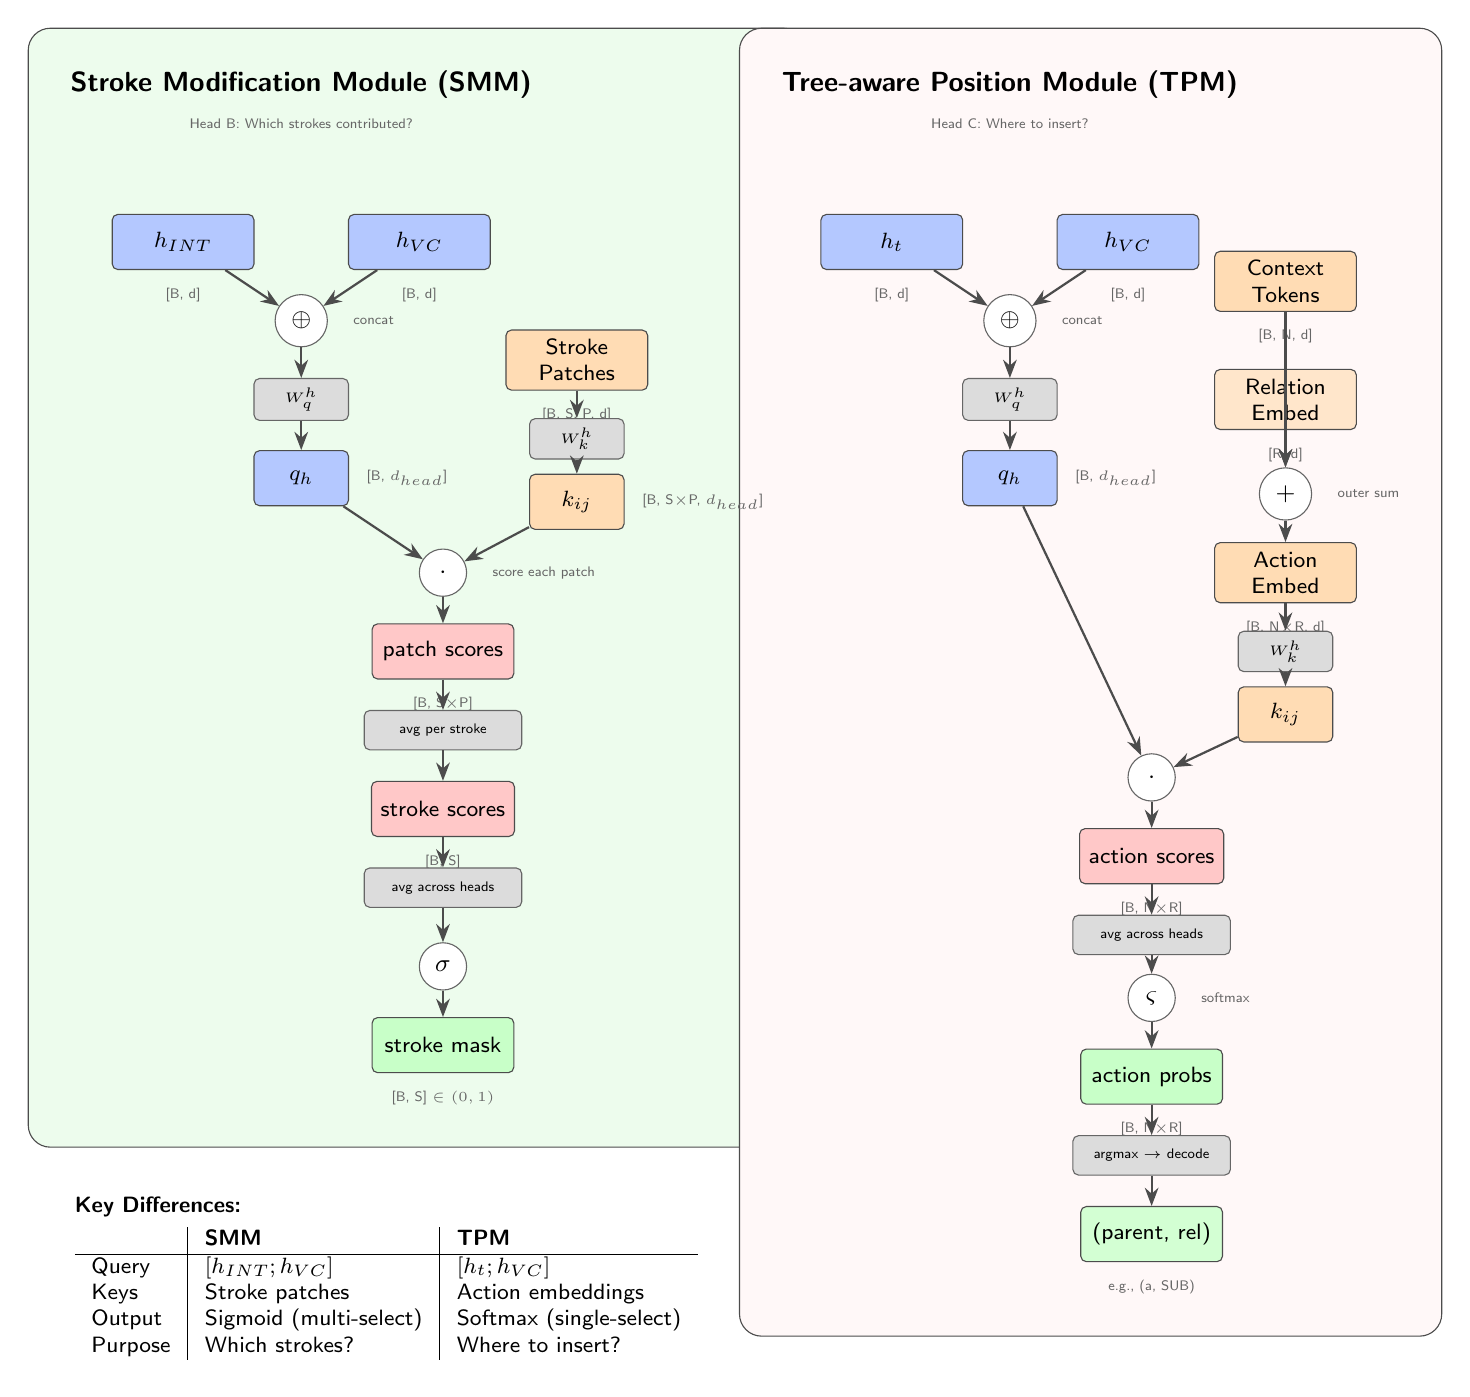
\begin{tikzpicture}[
    % Node styles
    tensor/.style={
        rectangle, 
        draw=black!70, 
        fill=#1, 
        rounded corners=2pt,
        minimum width=1.8cm, 
        minimum height=0.7cm,
        font=\footnotesize\sffamily,
        align=center
    },
    tensor/.default=white,
    proj/.style={
        rectangle, 
        draw=black!60, 
        fill=projcolor, 
        rounded corners=2pt,
        minimum width=1.2cm, 
        minimum height=0.5cm,
        font=\tiny\sffamily
    },
    op/.style={
        circle,
        draw=black!60,
        fill=white,
        minimum size=0.6cm,
        font=\small\sffamily
    },
    module/.style={
        rectangle, 
        draw=black!70, 
        fill=#1, 
        rounded corners=8pt,
        inner sep=12pt
    },
    arrow/.style={
        ->,
        >=Stealth,
        thick,
        black!70
    },
    label/.style={
        font=\tiny\sffamily,
        text=black!60
    }
]

% ============================================
% SMM MODULE (Left side)
% ============================================

\begin{scope}[local bounding box=smm_scope]
    
    % Module title
    \node[font=\normalsize\bfseries\sffamily] (smm_title) at (0, 5) {Stroke Modification Module (SMM)};
    \node[label] at (0, 4.5) {Head B: Which strokes contributed?};
    
    % Inputs
    \node[tensor=querycolor] (h_int) at (-1.5, 3) {$h_{INT}$};
    \node[tensor=querycolor] (h_vc_smm) at (1.5, 3) {$h_{VC}$};
    \node[label, below=0.1cm of h_int] {[B, d]};
    \node[label, below=0.1cm of h_vc_smm] {[B, d]};
    
    % Concat
    \node[op] (concat_smm) at (0, 2) {$\oplus$};
    \node[label, right=0.2cm of concat_smm] {concat};
    
    % Query projection
    \node[proj] (q_proj_smm) at (0, 1) {$W_q^h$};
    \node[tensor=querycolor, minimum width=1.2cm] (q_smm) at (0, 0) {$q_h$};
    \node[label, right=0.1cm of q_smm] {[B, $d_{head}$]};
    
    % Key input (stroke patches)
    \node[tensor=keycolor] (patches) at (3.5, 1.5) {Stroke\\Patches};
    \node[label, below=0.1cm of patches] {[B, S, P, d]};
    
    % Key projection
    \node[proj] (k_proj_smm) at (3.5, 0.5) {$W_k^h$};
    \node[tensor=keycolor, minimum width=1.2cm] (k_smm) at (3.5, -0.3) {$k_{ij}$};
    \node[label, right=0.1cm of k_smm] {[B, S$\times$P, $d_{head}$]};
    
    % Dot product
    \node[op] (dot_smm) at (1.8, -1.2) {$\cdot$};
    \node[label, right=0.2cm of dot_smm] {score each patch};
    
    % Per-patch scores
    \node[tensor=scorecolor] (patch_scores) at (1.8, -2.2) {patch scores};
    \node[label, below=0.1cm of patch_scores] {[B, S$\times$P]};
    
    % Average within stroke
    \node[proj, minimum width=2cm] (avg_stroke) at (1.8, -3.2) {avg per stroke};
    
    % Stroke scores
    \node[tensor=scorecolor] (stroke_scores) at (1.8, -4.2) {stroke scores};
    \node[label, below=0.1cm of stroke_scores] {[B, S]};
    
    % Average across heads
    \node[proj, minimum width=2cm] (avg_heads) at (1.8, -5.2) {avg across heads};
    
    % Sigmoid
    \node[op] (sigmoid) at (1.8, -6.2) {$\sigma$};
    
    % Output
    \node[tensor=outputcolor] (out_smm) at (1.8, -7.2) {stroke mask};
    \node[label, below=0.1cm of out_smm] {[B, S] $\in (0,1)$};
    
    % Arrows
    \draw[arrow] (h_int) -- (concat_smm);
    \draw[arrow] (h_vc_smm) -- (concat_smm);
    \draw[arrow] (concat_smm) -- (q_proj_smm);
    \draw[arrow] (q_proj_smm) -- (q_smm);
    \draw[arrow] (patches) -- (k_proj_smm);
    \draw[arrow] (k_proj_smm) -- (k_smm);
    \draw[arrow] (q_smm) -- (dot_smm);
    \draw[arrow] (k_smm) -- (dot_smm);
    \draw[arrow] (dot_smm) -- (patch_scores);
    \draw[arrow] (patch_scores) -- (avg_stroke);
    \draw[arrow] (avg_stroke) -- (stroke_scores);
    \draw[arrow] (stroke_scores) -- (avg_heads);
    \draw[arrow] (avg_heads) -- (sigmoid);
    \draw[arrow] (sigmoid) -- (out_smm);

\end{scope}

% SMM background
\begin{scope}[on background layer]
    \node[module=modulegreen!50, fit=(smm_scope)] {};
\end{scope}

% ============================================
% TPM MODULE (Right side)
% ============================================

\begin{scope}[local bounding box=tpm_scope, xshift=9cm]
    
    % Module title
    \node[font=\normalsize\bfseries\sffamily] (tpm_title) at (0, 5) {Tree-aware Position Module (TPM)};
    \node[label] at (0, 4.5) {Head C: Where to insert?};
    
    % Inputs
    \node[tensor=querycolor] (h_t) at (-1.5, 3) {$h_t$};
    \node[tensor=querycolor] (h_vc_tpm) at (1.5, 3) {$h_{VC}$};
    \node[label, below=0.1cm of h_t] {[B, d]};
    \node[label, below=0.1cm of h_vc_tpm] {[B, d]};
    
    % Concat
    \node[op] (concat_tpm) at (0, 2) {$\oplus$};
    \node[label, right=0.2cm of concat_tpm] {concat};
    
    % Query projection
    \node[proj] (q_proj_tpm) at (0, 1) {$W_q^h$};
    \node[tensor=querycolor, minimum width=1.2cm] (q_tpm) at (0, 0) {$q_h$};
    \node[label, right=0.1cm of q_tpm] {[B, $d_{head}$]};
    
    % Key inputs (context + relation)
    \node[tensor=keycolor] (ctx_emb) at (3.5, 2.5) {Context\\Tokens};
    \node[label, below=0.1cm of ctx_emb] {[B, N, d]};
    
    \node[tensor=keycolor!70] (rel_emb) at (3.5, 1) {Relation\\Embed};
    \node[label, below=0.1cm of rel_emb] {[R, d]};
    
    % Plus for action embeddings
    \node[op] (plus_action) at (3.5, -0.2) {$+$};
    \node[label, right=0.2cm of plus_action] {outer sum};
    
    % Action embeddings
    \node[tensor=keycolor] (action_emb) at (3.5, -1.2) {Action\\Embed};
    \node[label, below=0.1cm of action_emb] {[B, N$\times$R, d]};
    
    % Key projection
    \node[proj] (k_proj_tpm) at (3.5, -2.2) {$W_k^h$};
    \node[tensor=keycolor, minimum width=1.2cm] (k_tpm) at (3.5, -3) {$k_{ij}$};
    
    % Dot product
    \node[op] (dot_tpm) at (1.8, -3.8) {$\cdot$};
    
    % Scores
    \node[tensor=scorecolor] (action_scores) at (1.8, -4.8) {action scores};
    \node[label, below=0.1cm of action_scores] {[B, N$\times$R]};
    
    % Average across heads
    \node[proj, minimum width=2cm] (avg_heads_tpm) at (1.8, -5.8) {avg across heads};
    
    % Softmax
    \node[op] (softmax) at (1.8, -6.6) {$\varsigma$};
    \node[label, right=0.2cm of softmax] {softmax};
    
    % Output
    \node[tensor=outputcolor] (out_tpm) at (1.8, -7.6) {action probs};
    \node[label, below=0.1cm of out_tpm] {[B, N$\times$R]};
    
    % Decode
    \node[proj, minimum width=2cm] (decode) at (1.8, -8.6) {argmax $\rightarrow$ decode};
    
    % Final output
    \node[tensor=outputcolor!80] (final_out) at (1.8, -9.6) {(parent, rel)};
    \node[label, below=0.1cm of final_out] {e.g., (a, SUB)};
    
    % Arrows
    \draw[arrow] (h_t) -- (concat_tpm);
    \draw[arrow] (h_vc_tpm) -- (concat_tpm);
    \draw[arrow] (concat_tpm) -- (q_proj_tpm);
    \draw[arrow] (q_proj_tpm) -- (q_tpm);
    \draw[arrow] (ctx_emb) -- (plus_action);
    \draw[arrow] (rel_emb) -- (plus_action);
    \draw[arrow] (plus_action) -- (action_emb);
    \draw[arrow] (action_emb) -- (k_proj_tpm);
    \draw[arrow] (k_proj_tpm) -- (k_tpm);
    \draw[arrow] (q_tpm) -- (dot_tpm);
    \draw[arrow] (k_tpm) -- (dot_tpm);
    \draw[arrow] (dot_tpm) -- (action_scores);
    \draw[arrow] (action_scores) -- (avg_heads_tpm);
    \draw[arrow] (avg_heads_tpm) -- (softmax);
    \draw[arrow] (softmax) -- (out_tpm);
    \draw[arrow] (out_tpm) -- (decode);
    \draw[arrow] (decode) -- (final_out);

\end{scope}

% TPM background
\begin{scope}[on background layer]
    \node[module=modulepink!50, fit=(tpm_scope)] {};
\end{scope}

% ============================================
% COMPARISON TABLE (Bottom)
% ============================================

\node[
    font=\footnotesize\sffamily,
    align=left,
    anchor=north west
] at (-3, -9) {
    \textbf{Key Differences:}\\[3pt]
    \begin{tabular}{l|l|l}
        & \textbf{SMM} & \textbf{TPM} \\
        \hline
        Query & $[h_{INT}; h_{VC}]$ & $[h_t; h_{VC}]$ \\
        Keys & Stroke patches & Action embeddings \\
        Output & Sigmoid (multi-select) & Softmax (single-select) \\
        Purpose & Which strokes? & Where to insert? \\
    \end{tabular}
};

\end{tikzpicture}

\end{document}

